\documentclass[a4paper]{article}

\usepackage{authblk}
\usepackage{kotex, amsmath,amssymb,amsthm, mathtools, physics}
\usepackage{tikz,titlesec,hyperref, enumitem, systeme, bbm}
\usepackage{csquotes}
\usepackage[ruled,vlined]{algorithm2e}
\usepackage{optidef}
\usepackage{arydshln}
\usepackage{xcolor}
%\usepackage{subfig}
\usepackage[normalem]{ulem}
\usepackage{booktabs}
\usepackage{courier}
\usepackage{tabularx, environ}
\usepackage{subfigure}
\usepackage{graphicx}
\usepackage{float}
\usepackage[numbib]{tocbibind}


\newtheorem{theorem}{Theorem}[section]
\newtheorem{conjecture}{Conjecture}[theorem]
\newtheorem{corollary}{Corollary}[theorem]
\newtheorem{lemma}[theorem]{Lemma}

\newtheorem*{remark}{Remark}

\usepackage[a4paper,margin=2cm]{geometry}

\linespread{1.3}

\newtheorem{claim}{Claim}[section]

\makeatletter
\newcommand{\problemtitle}[1]{\gdef\@problemtitle{#1}}% Store problem title
\newcommand{\probleminput}[1]{\gdef\@probleminput{#1}}% Store problem input
\newcommand{\problemquestion}[1]{\gdef\@problemquestion{#1}}% Store problem question
\NewEnviron{problem}{
	\problemtitle{}\probleminput{}\problemquestion{}% Default input is empty
	\BODY% Parse input
	\par\addvspace{.5\baselineskip}
	\noindent
	\begin{tabularx}{\textwidth}{@{\hspace{\parindent}} l X c}
		\multicolumn{2}{@{\hspace{\parindent}}l}{\@problemtitle} \\% Title
		\textbf{Input:} & \@probleminput \\% Input
		\textbf{Question:} & \@problemquestion% Question
	\end{tabularx}
	\par\addvspace{.5\baselineskip}
}
\makeatother

\newcommand\name{Junghyun Lee}   % Name of the student
\newcommand\university{KAIST} % Name of the university
\newcommand\department{Dept. of Mathematical Sciences \& School of Computing} % Name of the department
\newcommand\studentid{20170500} % Student ID
\newcommand\lastupdate{Last update: }

\title{(CS454) Assignment \#2: \\
	{\it Hybrid Optimisation for TSP} \bigskip}
\author{\textbf{\Large \name}\thanks{jh\_lee00@kaist.ac.kr} \ (\studentid) \\
\department, \university}
%\lastupdate \date{\today}
\date{\today}

\begin{document}
\thispagestyle{empty}
\maketitle
\tableofcontents
\newpage


%\begin{figure}[htp] 
%	\centering
%	\subfloat[A motivating example from the GTSRB dataset]{%
%		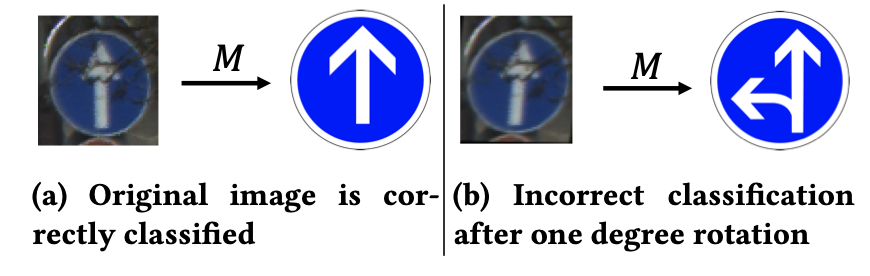
\includegraphics[width=0.46\textwidth]{fig1.png}%
%		\label{fig:1a}%
%	}%
%	\hfill%
%	\subfloat[An overview of \textsc{Sensei} for one seed image in one epoch.]{%
%		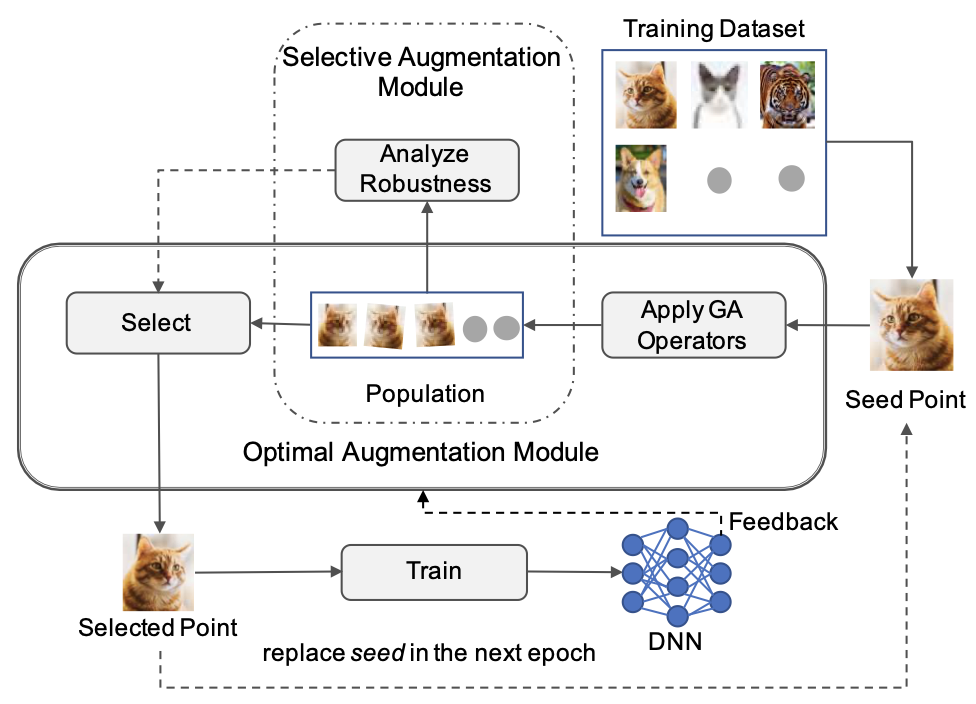
\includegraphics[width=0.46\textwidth]{fig3.png}%
%		\label{fig:1b}%
%	}%
%	\caption{Figures from \cite{GSPR20}}
%	\label{fig:1}
%\end{figure}


\section{Background}
This algorithm deals with the symmetric Euclidean travelling salesperson problem(TSP from here on forth)
The precise mathematical formulation is as follows:
\begin{problem}
%	\problemtitle{\textsc{TSP}}
	\probleminput{A set of $N$ coordinates $\{(x_i, y_i)\}_{i=0}^{N-1}$.}
	\problemquestion{Find the Hamiltonian cycle of $K_N$ with the least weight, where $K_N$ is a undirected complete graph on vertices $\{(x_i, y_i)\}_{i=0}^{N-1}$ whose edge weight is the usual Euclidean distance.}
\end{problem}

This problem is known to be NP-hard, and thus we need to resort to approximation algorithms.

Such algorithms can be divided into two types: stochastic and non-stochastic.
There are a vast amount of literature on both types of algorithms (see \cite{La92, Ma09, ABCC07} for an extensive survey of this)
This implementation makes uses of both types of algorithms, as explained in the next section.


\section{Algorithm}
Figure \ref{fig1} shows a very rough picture of this algorithm:
\begin{figure}
\label{fig1}
	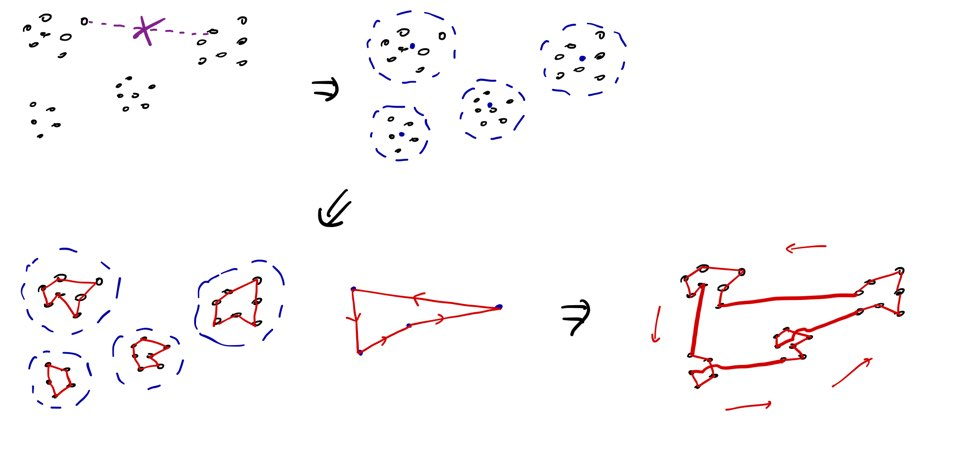
\includegraphics[width=\textwidth]{Figures/fig1.jpg}
	\caption{Rough picture of the algorithm}
\end{figure}
This section provides a step-by-step description of the algorithm, along with suitable justifications/motivations of each step.
Also, implementation details such as packages used are also provided.

\subsection{k-Means Clustering}
One of the most promising features of many global search meta-heuristics (such as GA, ACO, PSO...etc) is that they are applicable to almost any kind of optimization problems with no prior knowledge whatsoever: the objective function can even be blackbox.
However, this is why 
 not scalable; in other words, as the problem size grows, the trade-off between amount of required resources and quality of the solution worsens.
This is paradoxically partly due to the characteristic of such algorithms that they do not exploit any specific structures of the problems.
Thus I propose to use clustering as a \enquote{preprocessing} before applying the stochastic algorithms.
This allows for the algorithm to exploit the geometric feature of TSP: if points are clustered together, then they should be nearby in the optimal Hamiltonian cycle, and if points are far away, then they should be far apart.
My algorithm uses k-means clustering, implemented by \texttt{sklearn.cluster.KMeans}.
This creates local TSP problem instances, corresponding to each cluster.

\subsection{Intracluster ACOs}
Obviously, the next step is to solve each local TSPs.
I've used ACO (ant colony optimization), which was implemented by myself in \texttt{TSP\_ACO.py}.
Reason for selecting ACO is that along with GA, it was shown empirically to outperform other stochastic metaheuristics\cite{CT19}.
Also, (although not implemented), it is easier and more intuitive to apply hyperparameter tuning for the ACO instance. For more details, see Section \ref{subsec:hyper}
Hyperparameters used are as follows: $T = 100, k = 10, a = 1, b = 1, \rho = 0.1$\footnote{$T$: maximum iterations, $k$: number of ants, $a, b$: exponents determining the dependency of the probability distribution on edge distance and pheromone deposit, $\rho$: pheromone evaporation ratio}.
(Same formulation of the ACO as discussed in the class was used)
This creates a partition of the complete graph(induced by the input coordinates) into $n$ cycles, where $n$ is the number of clusters.
One obvious trick to accelerate this process is described:

\subsubsection{Parallelizing these ACOs}
Note that each cluster's TSP is independent of another, which means that this can be parallelized.
However, in current implementation, this was not possible.
For the detailed reason, refer to the Section \ref{subsubsec:parallel}.


\subsection{Intercluster ACO}
In order to combine the local solutions, produced by previous step, the algorithm solves a TSP instance, created by the medians of the clusters.
Weaker setting for ACO was used: $T = 50, k = 5, a = 1, b = 1, \rho = 0.1$.


\subsection{Combine the local solutions into a global solutions}
Based on the order of the clusters as found previously, the algorithm combines all local solutions into a global solution in a greedy manner.
Figure \ref{fig2} and \ref{fig3} illustrates how this is implemented.
\begin{figure}[htp]
	\centering
	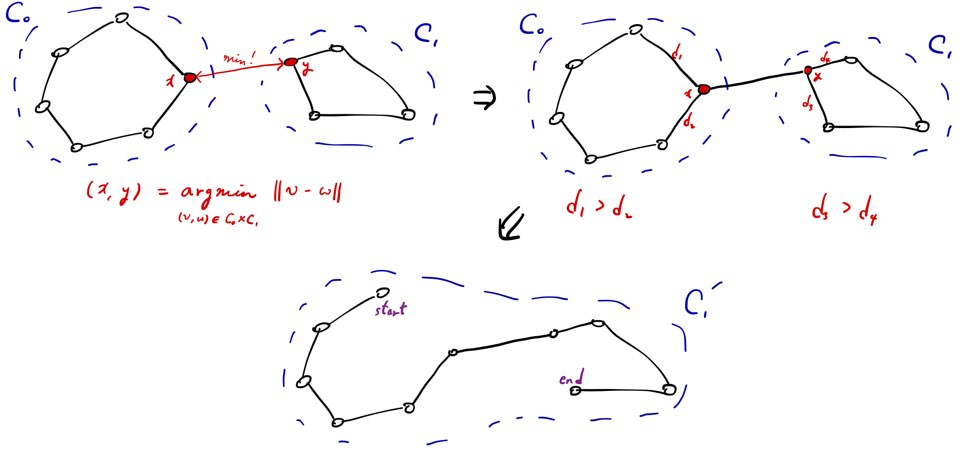
\includegraphics[width=\textwidth]{Figures/fig2.jpg}
	\caption{Initialization}
	\label{fig2}
	
	\vspace{2cm}% https://tex.stackexchange.com/q/26521/5764
	
	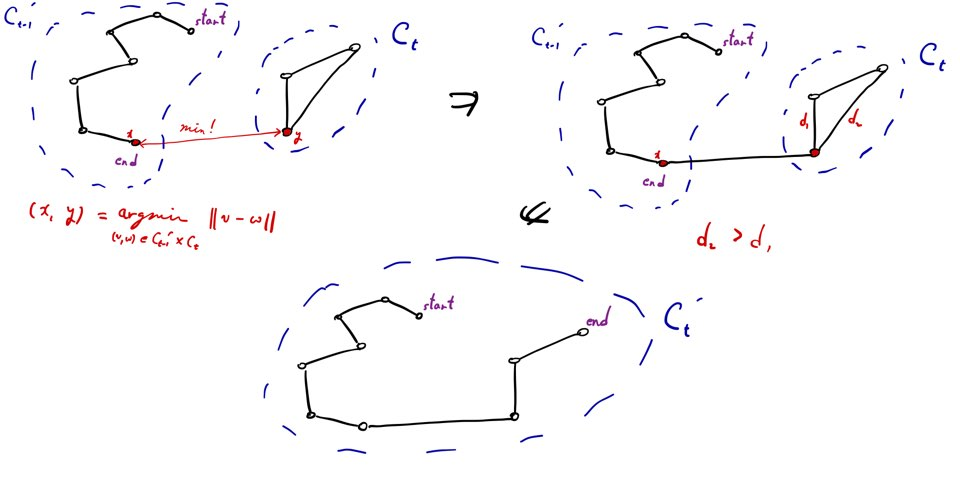
\includegraphics[width=\textwidth]{Figures/fig3.jpg}
	\caption{Rest of the iterations}
	\label{fig3}
	
\end{figure}
\begin{figure}
\centering
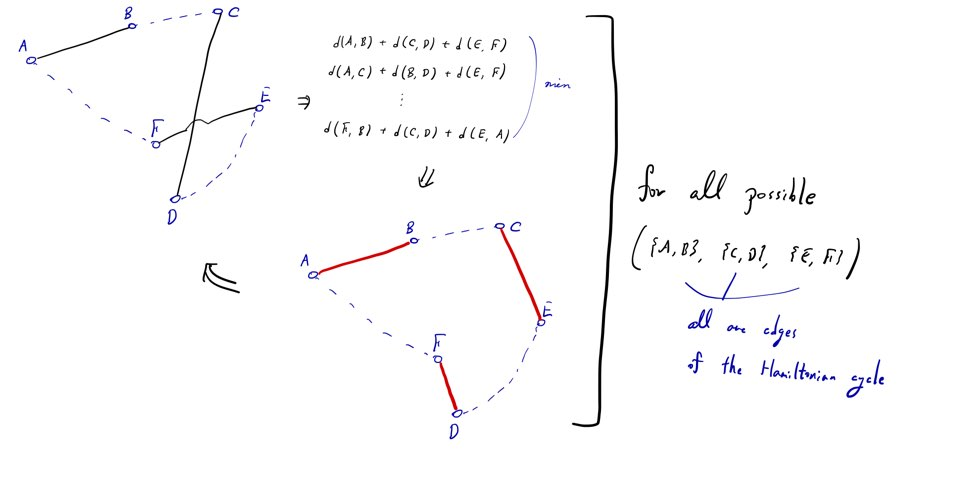
\includegraphics[width=\textwidth]{Figures/fig4.jpg}
\caption{Overview of 3-Opt Heuristic}
\label{fig4}
\end{figure}

\subsection{(*) 3-Opt Algorithm}
Many of the meta-heuristics available (including used ACO) may fall into some kind of a local minimum.
To escape from this, the algorithm performs 3-Opt heuristic.
Refer to Figure \ref{fig4} for the algorithmic details.
The locations (in the algorithm) of where the 3-Opt heuristic was performed are determined by the option \texttt{-topt}, of which is explained in Section {\ref{sec:usage}.

Although not reported in this report, extensive experiments show that using 3-Opt in any ways improves the qualities of intermediate solutions produced (and thus improving the final solution's quality, overall) significantly.

\begin{remark}
	The Python implementation of the 3-Opt algorithm used is based upon the Wikipedia article\footnote{\hyperlink{https://en.wikipedia.org/wiki/3-opt}{https://en.wikipedia.org/wiki/3-opt}} of the same name.
\end{remark}


\subsection{(*) Number of clusters}
As one could guess, the number of clusters probably has a huge effect on the quality of the solution.
Indeed, as reported in Section \ref{subsec:rq1}, in the current implementation, the solution quality seems to have no discernible relationship; in other words, searching through all possible numbers of clusters is the best option that we have.


\section{Experiments}
To see the effectiveness of this algorithm, I've done several experiments.
The computing environment used is my laptop, which is $2.3$ GHz $8$-Core Intel Core i9 with $32$GB RAM.
$11$ TSP instances from TSPLIB\cite{Rei91} were used, all of which has known optimal solution.

\subsection{RQ1: Effect of number of clusters}
\label{subsec:rq1}
Figure \ref{fig5} and \ref{fig6} shows the effect of number of clusters on the quality of the solution produced, for each dataset considered.
Note that the overall behaviours are all random, and depending on the number of clusters, the quality of the solution changes greatly.
This is one of the disadvantages of the current implementation.

\begin{center}
	\begin{figure}[H]%
		\centering
		\subfigure[][]{%
			\label{fig6-a}%
			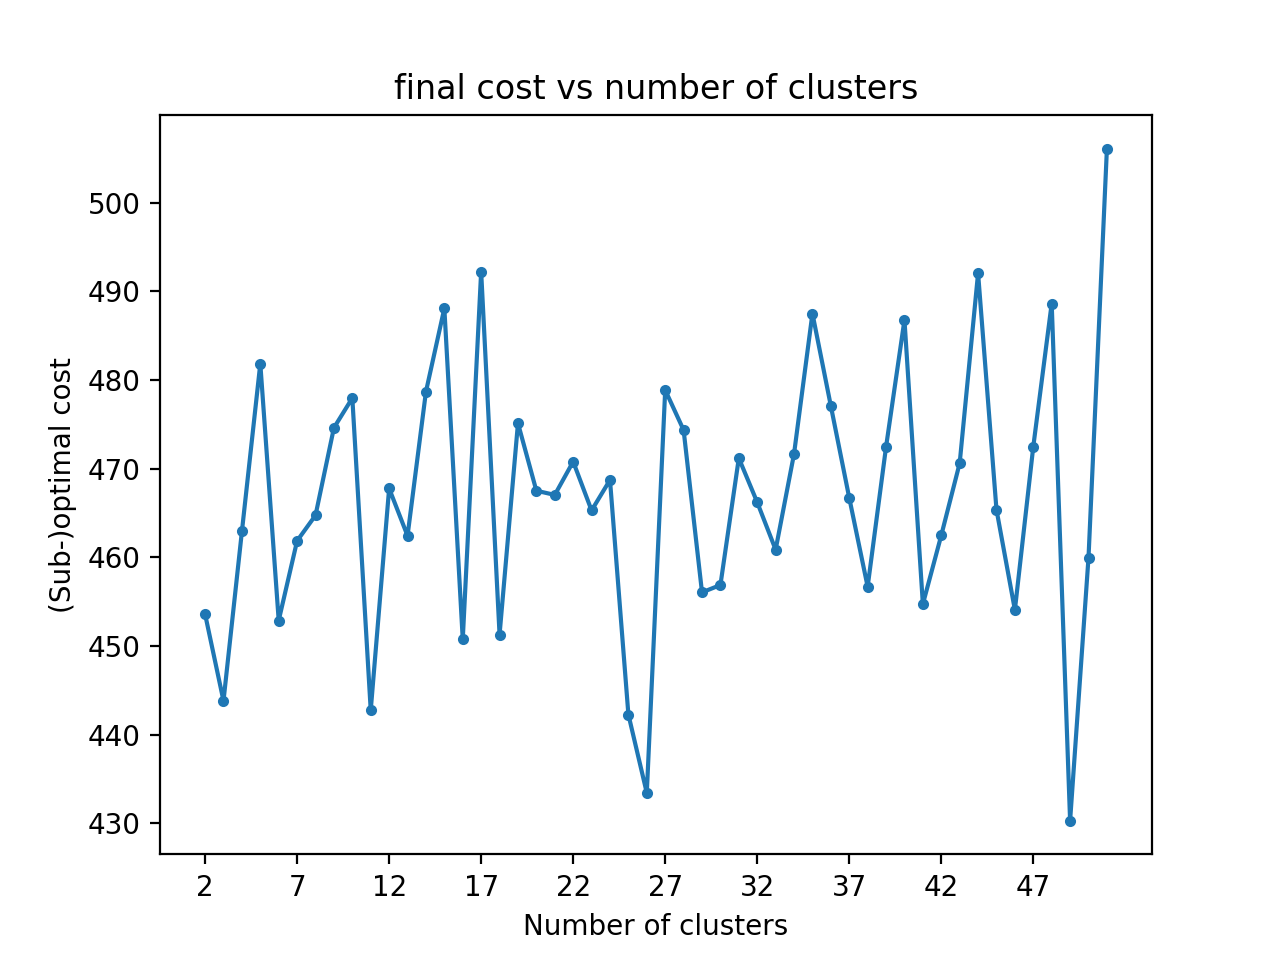
\includegraphics[width=0.4\textwidth]{Plots/eil51.png}}
		\hspace{8pt}%
		\subfigure[][]{%
			\label{fig6-b}%
			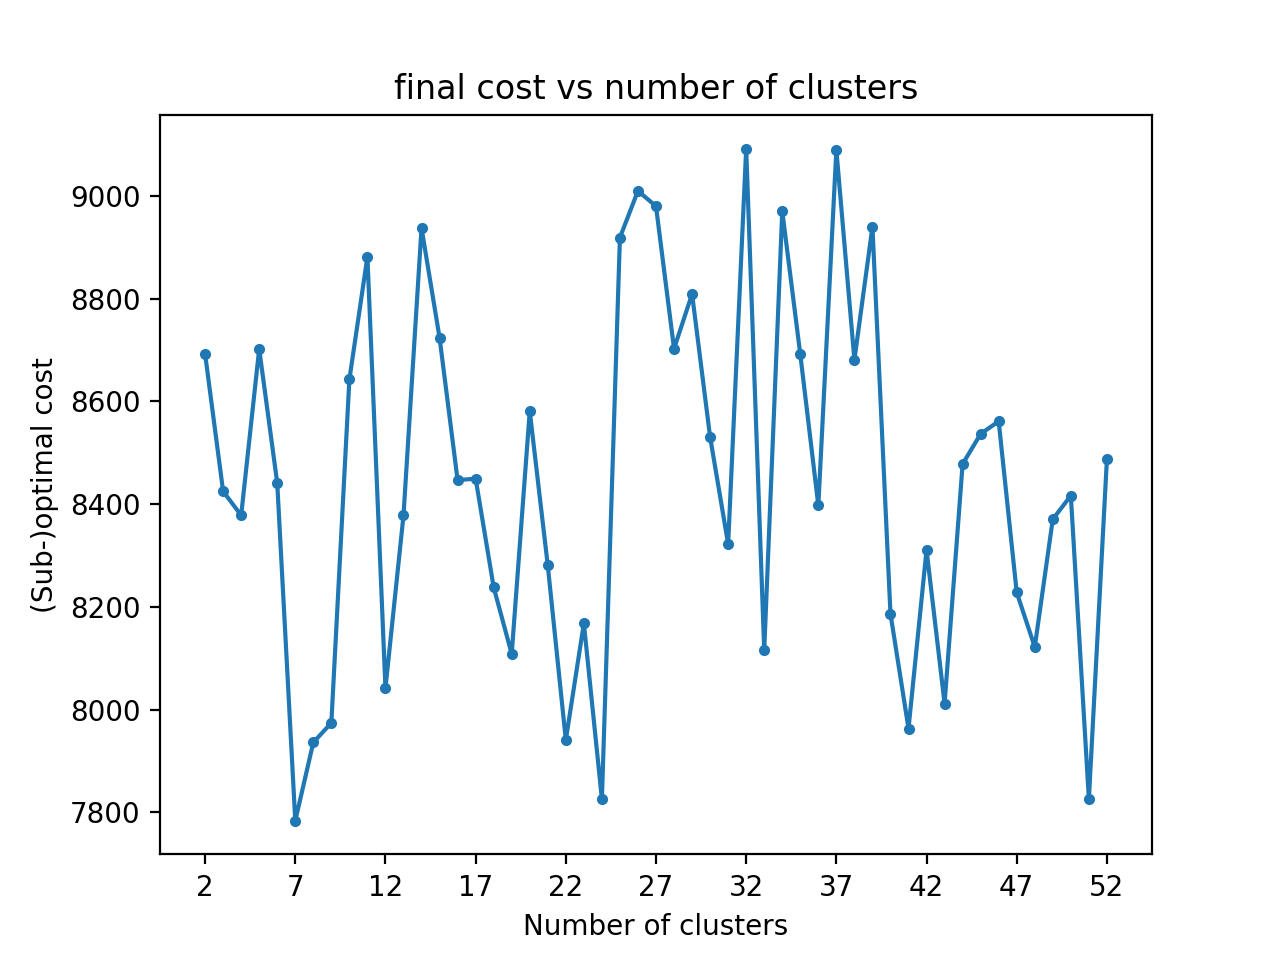
\includegraphics[width=0.4\textwidth]{Plots/berlin52.png}} \\
		\subfigure[][]{%
			\label{fig6-c}%
			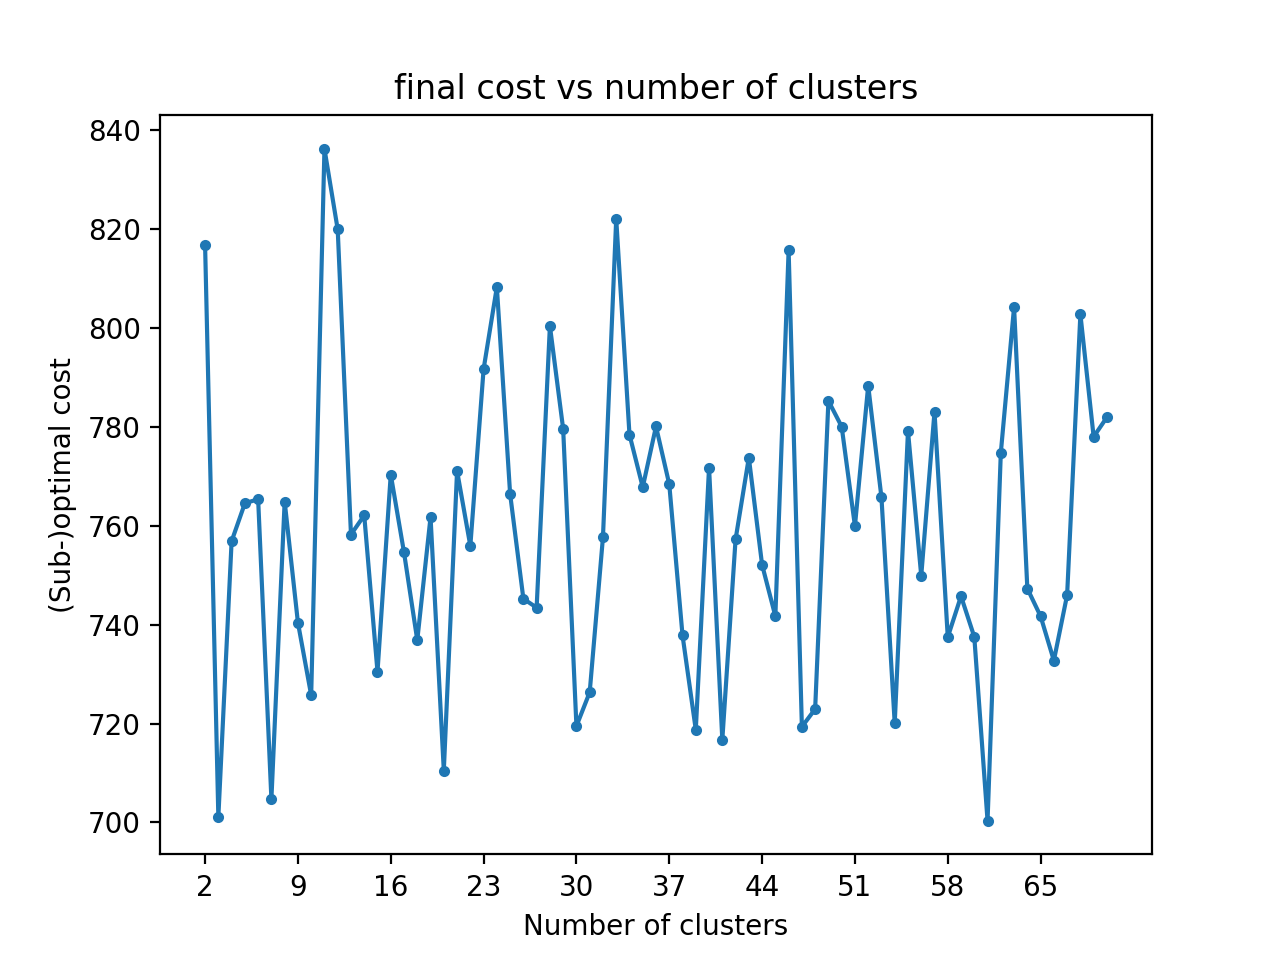
\includegraphics[width=0.4\textwidth]{Plots/st70.png}}%
		\hspace{8pt}%
		\subfigure[][]{%
			\label{fig6-d}%
			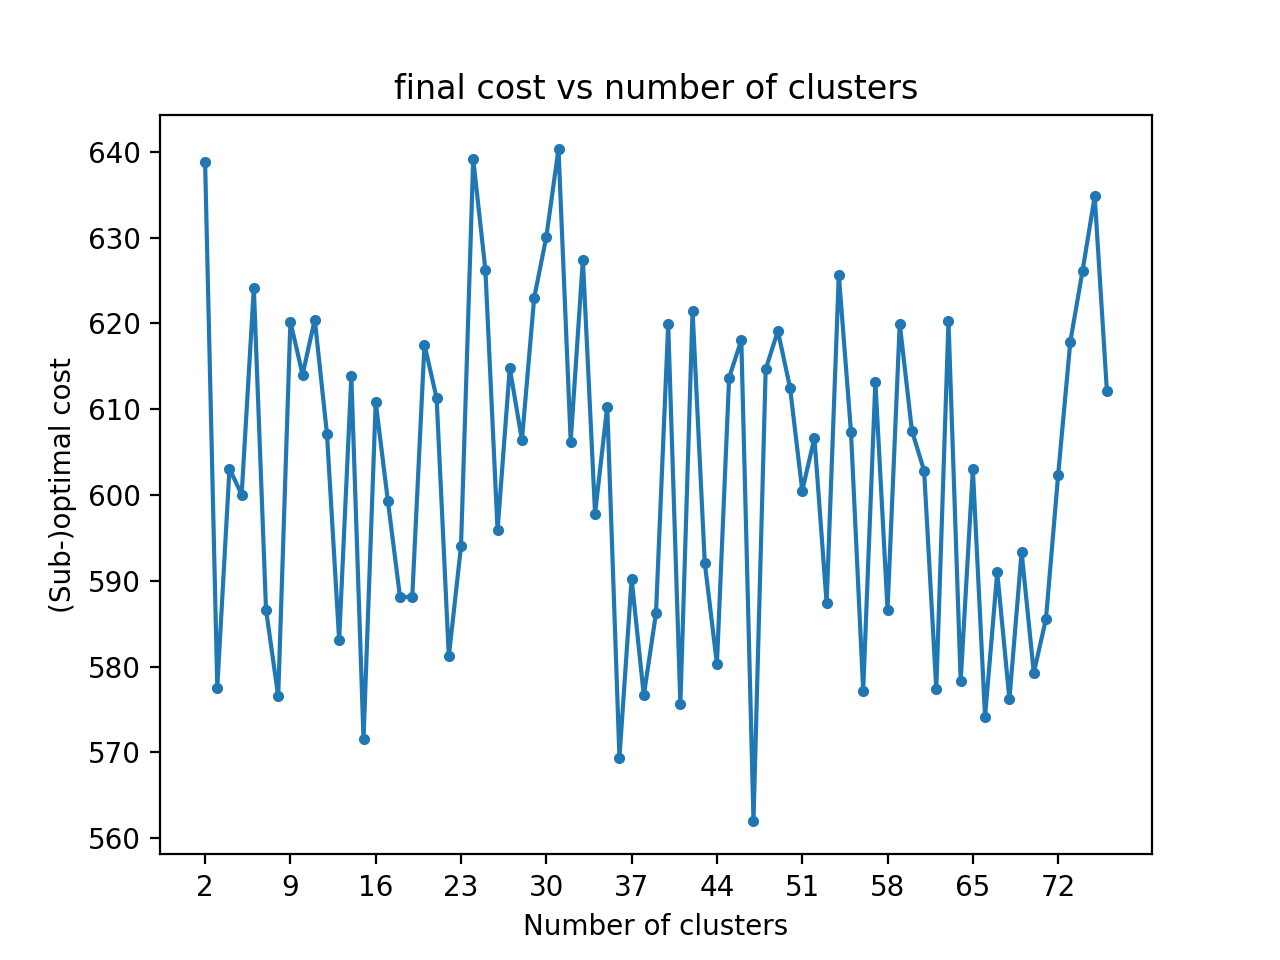
\includegraphics[width=0.4\textwidth]{Plots/eil76.png}} \\
		
		\caption[]{Datasets: (a) eil51.tsp (b) berlin52.tsp (c) st70.tsp (d) eil76.tsp }%
		\label{fig6}%
	\end{figure}
\end{center}
\begin{center}
\begin{figure}[H]%
	\centering
	\subfigure[][]{%
		\label{fig7-a}%
		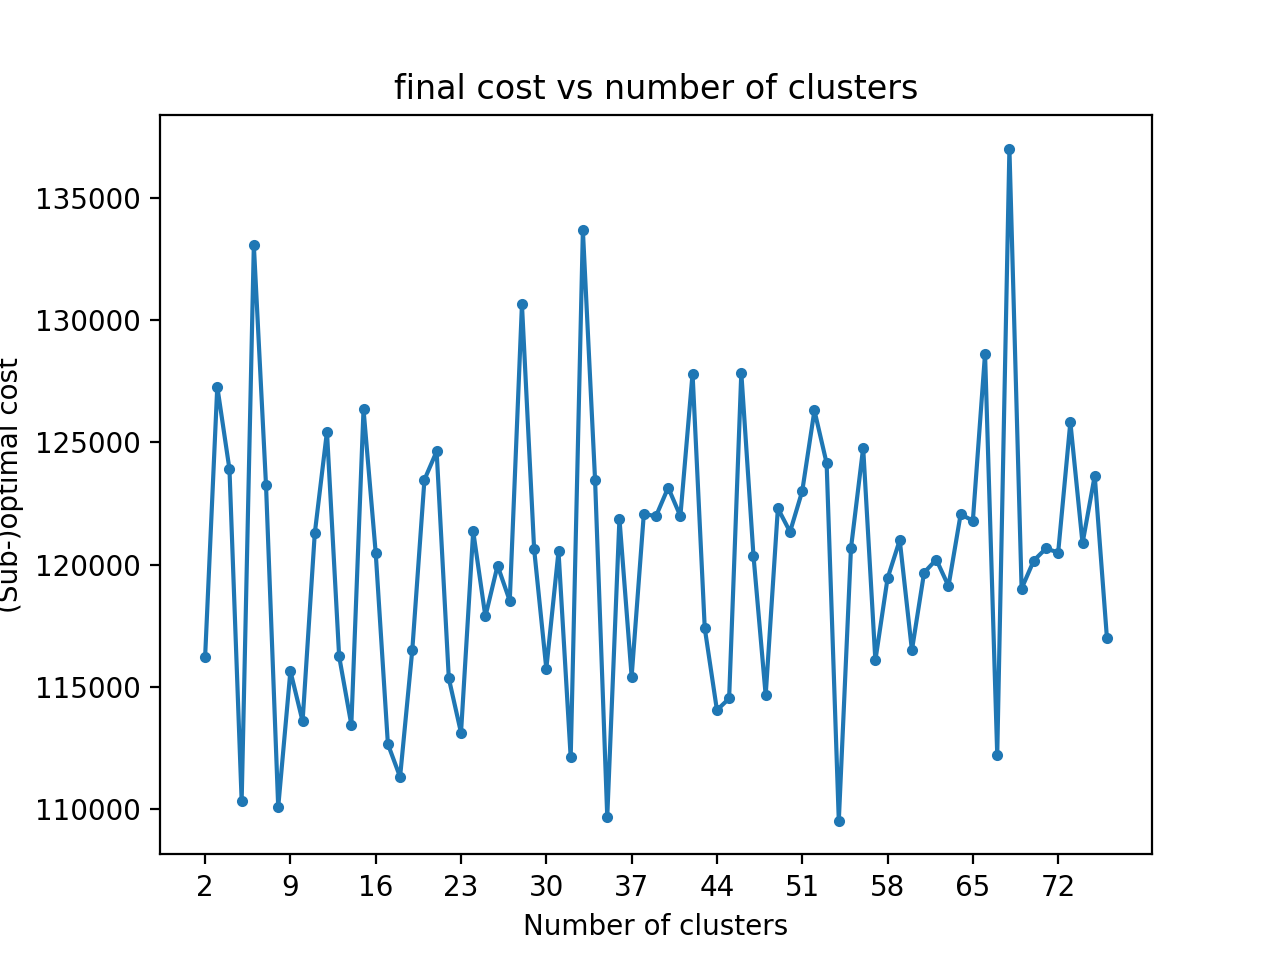
\includegraphics[width=0.4\textwidth]{Plots/pr76.png}}%
	\hspace{8pt}%
	\subfigure[][]{%
		\label{fig7-b}%
		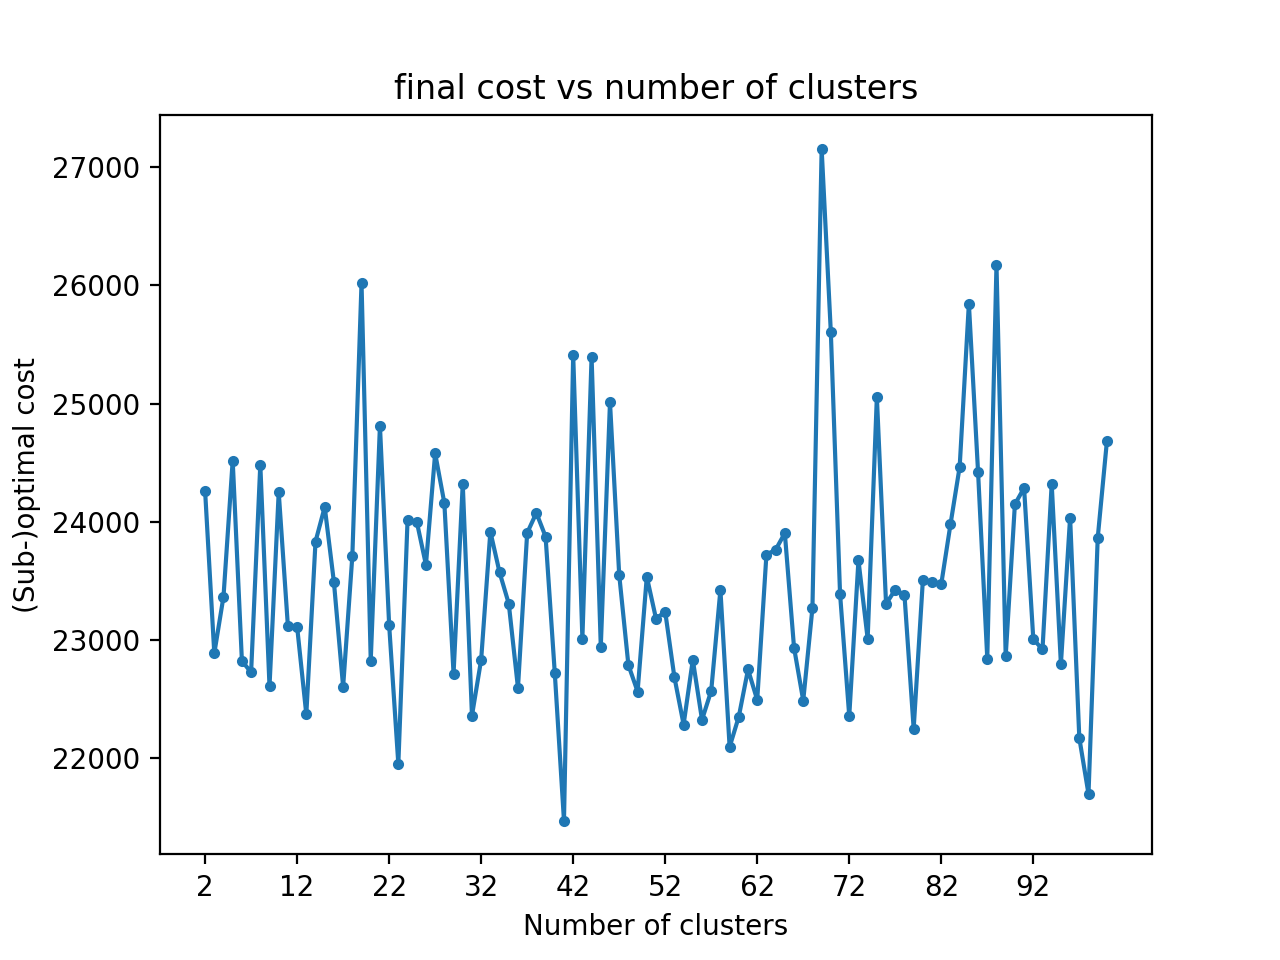
\includegraphics[width=0.4\textwidth]{Plots/kroa100.png}} \\
	\subfigure[][]{%
		\label{fig7-c}%
		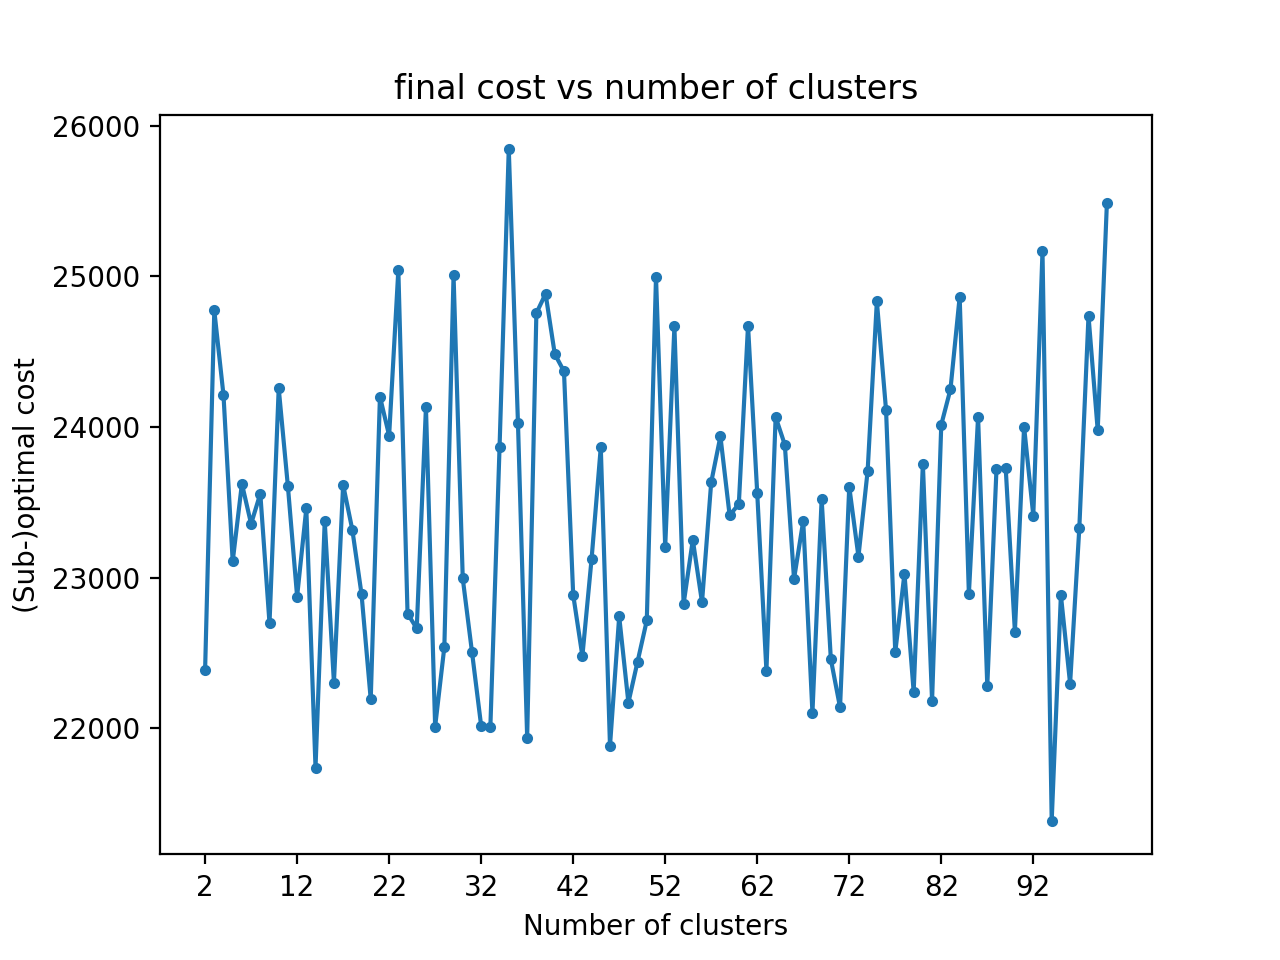
\includegraphics[width=0.4\textwidth]{Plots/kroc100.png}}%
	\hspace{8pt}%
	\subfigure[][]{%
		\label{fig7-d}%
		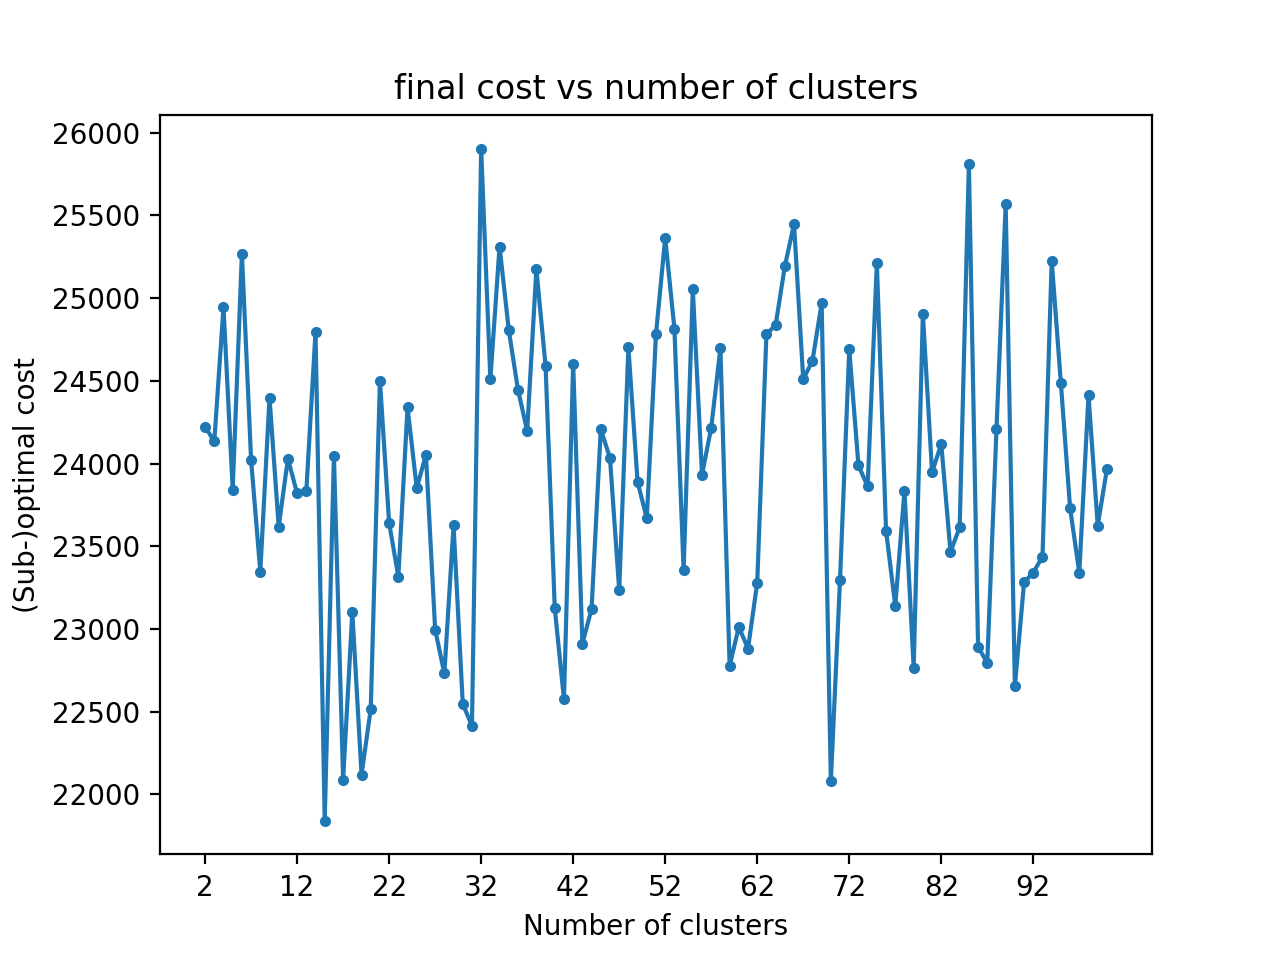
\includegraphics[width=0.4\textwidth]{Plots/krod100.png}} \\
		\subfigure[][]{%
		\label{fig7-e}%
		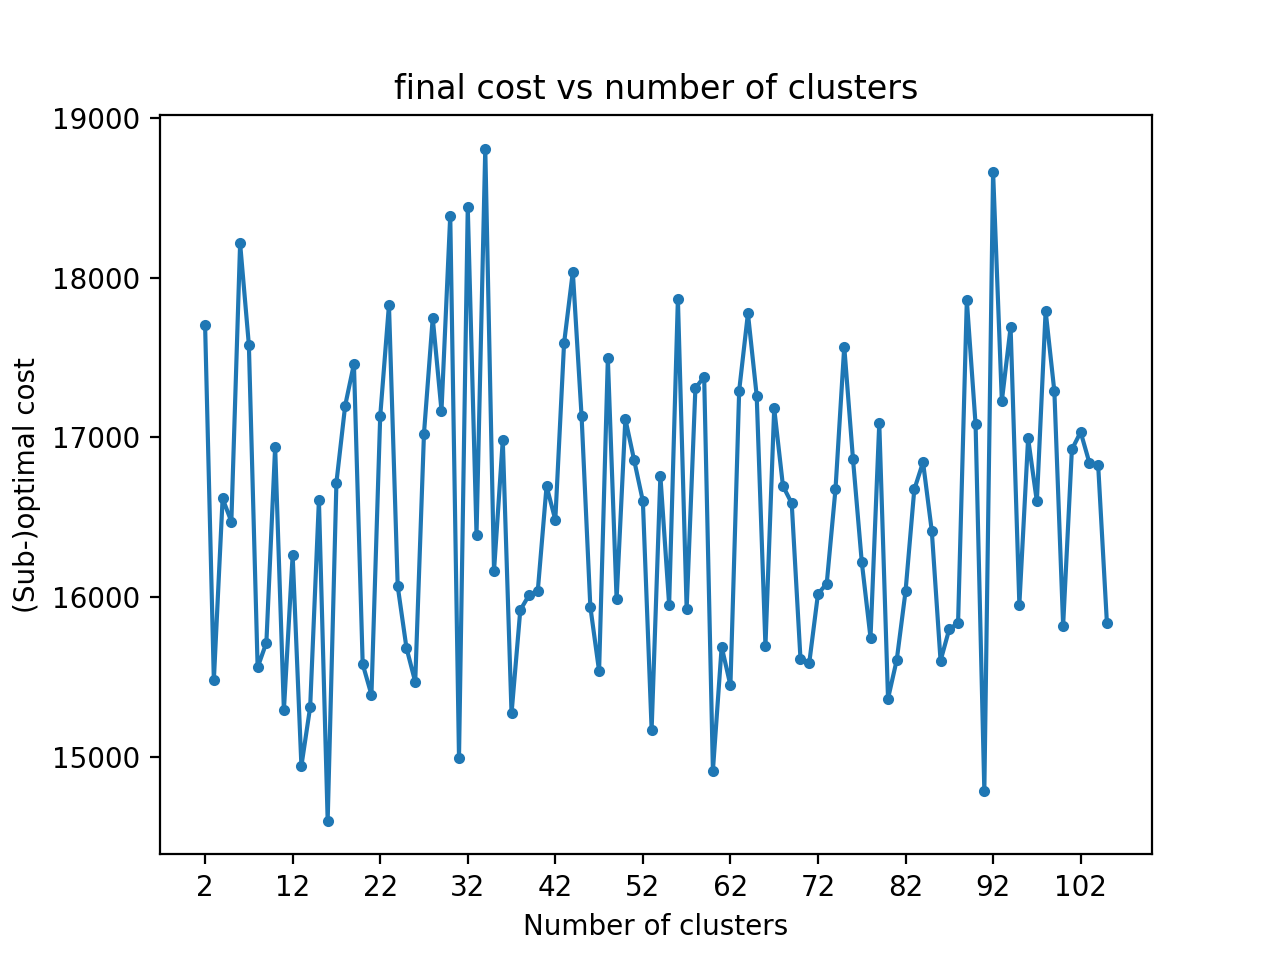
\includegraphics[width=0.4\textwidth]{Plots/lin105.png}}
	\hspace{8pt}%
	\subfigure[][]{%
		\label{fig7-f}%
		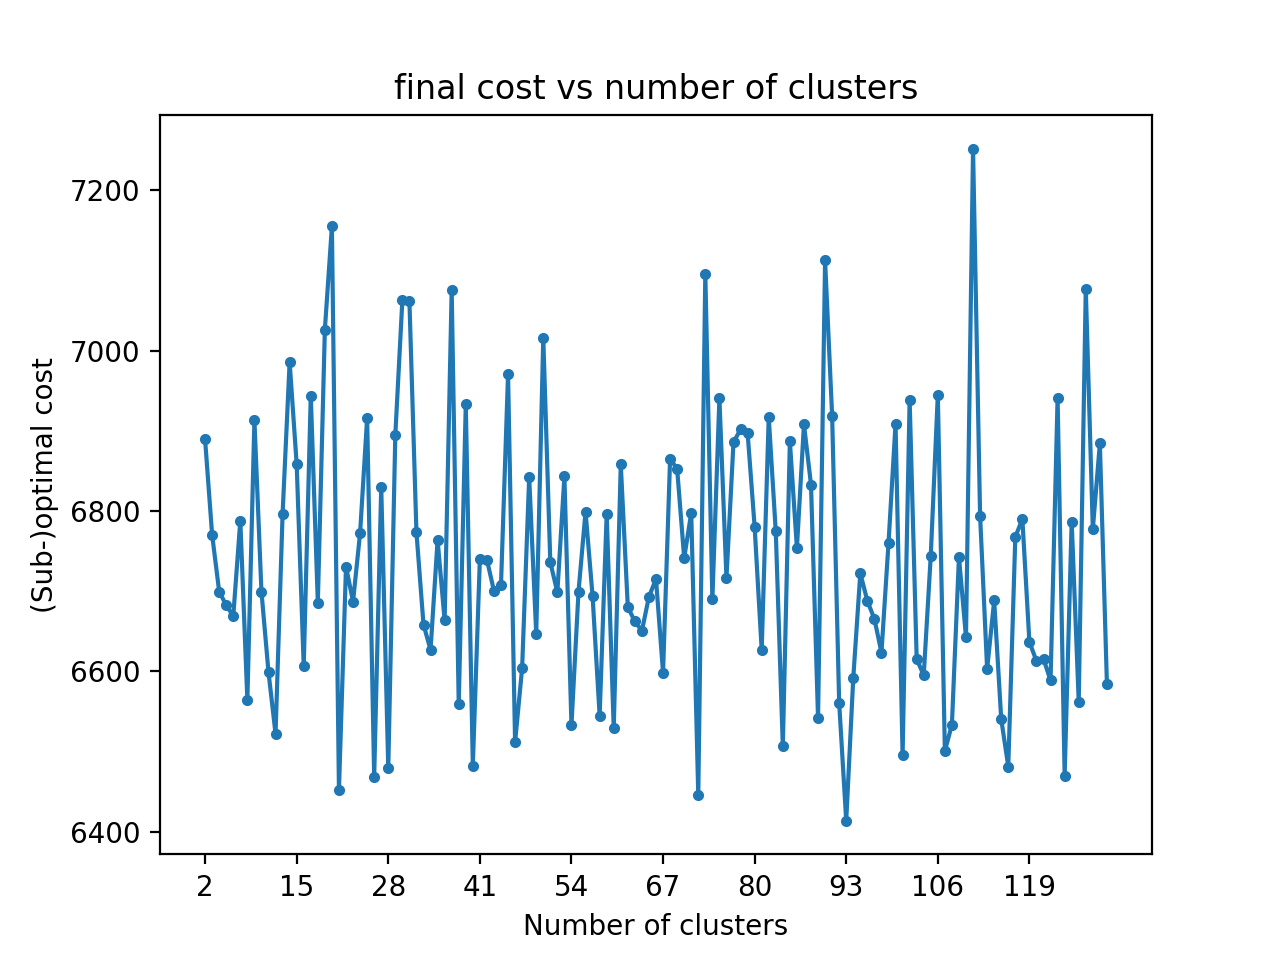
\includegraphics[width=0.4\textwidth]{Plots/ch130.png}} \\
	\subfigure[][]{%
		\label{fig7-g}%
		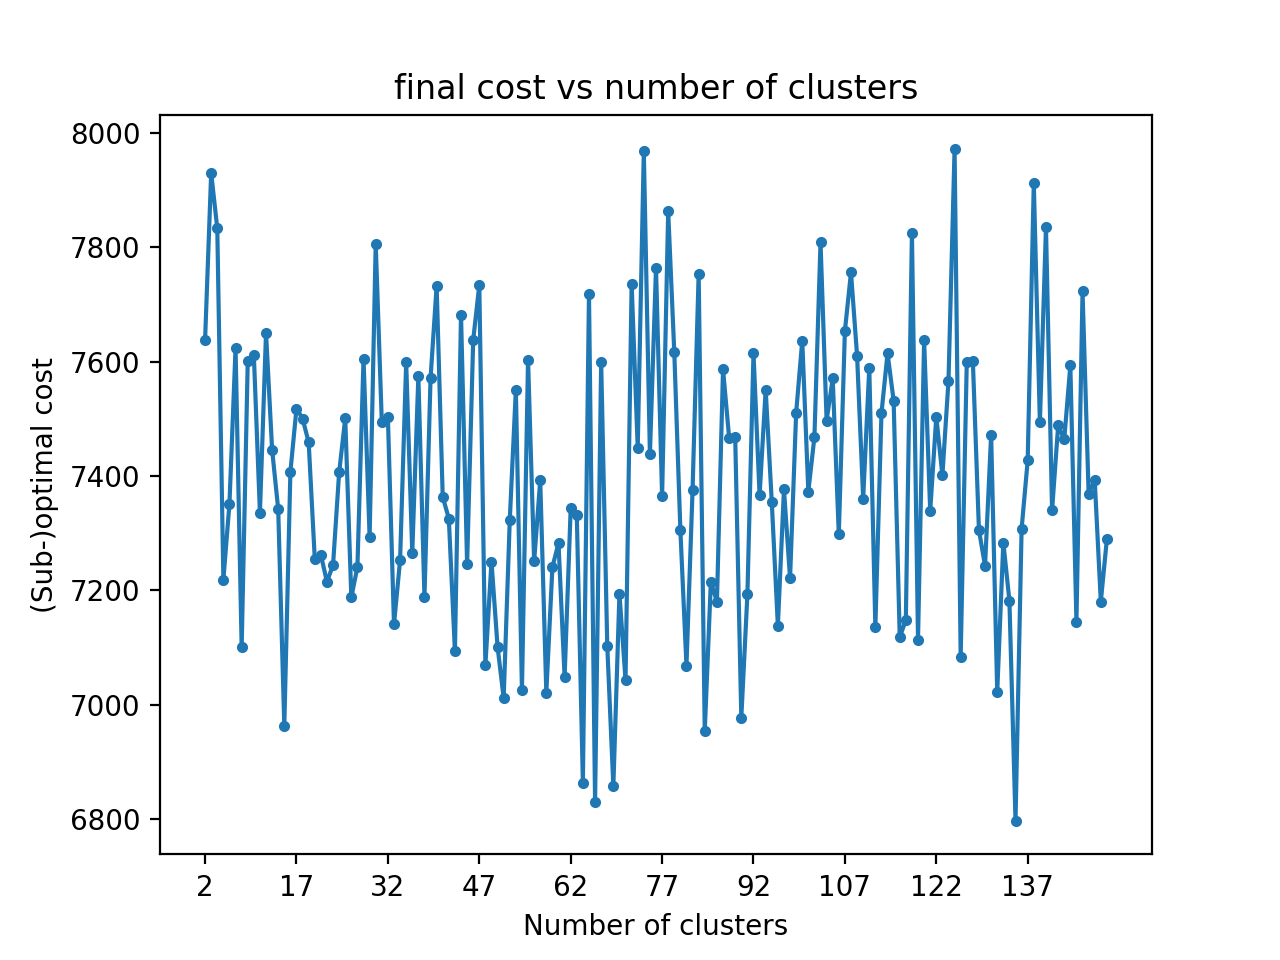
\includegraphics[width=0.4\textwidth]{Plots/ch150.png}}
%	\hspace{8pt}%
%	\subfigure[][]{%
%		\label{fig7-h}%
%		\includegraphics[width=0.4\textwidth]{Plots/tsp225.png}} \\
	
	\caption[]{Datasets: (a) pr76.tsp (b) kroa100.tsp (c) kroc100.tsp (d) krod100.tsp (e) lin105.tsp (f) ch130.tsp (g) ch150.tsp}%
	\label{fig5}%
\end{figure}
\end{center}


\subsection{RQ2: Performance of this algorithm}
Metric used to test the performance is the following:
\[ \left( 100 * \frac{resulting\_cost - optimal\_cost}{optimal\_cost} \right)\% \]

\begin{table*}[t!]
	\caption{All results (Datasets in increasing order of the instance size)}
	\label{table:results}
	\vskip 0.15in
	\begin{center}
		\begin{small}
			\begin{sc}
				\begin{tabular}{l|cccr}
					\toprule
					Dataset & Rel error(\%) & Runtime(sec) & Optimal \#clusters \\ \midrule
					eil51.tsp & 0.073571 & 21.168900 & 49 \\
					berlin52.tsp & 4.057245 & 23.480566 & 7 \\
					st70.tsp & 3.203759 & 70.912842 & 61 \\
					eil76.tsp & 3.050332 & 90.077797 & 47 \\
					pr76.tsp & 1.256251 & 99.081978 & 54 \\
					kroa100.tsp & 0.877605 & 292.646285 & 41 \\
					kroc100.tsp & 3.058841 & 297.441060 & 94 \\
					krod100.tsp & 2.567050 & 294.111822 & 15 \\
					lin105.tsp & 1.493876 & 341.559732 & 16 \\
					ch130.tsp & 4.958434 & 787.219632 & 93 \\
					ch150.tsp & 4.056542 & 1421.423156 & 135 \\
%					tsp225.tsp &  &  &  \\
					\bottomrule
				\end{tabular}
			\end{sc}
		\end{small}
	\end{center}
	\vskip -0.1in
\end{table*}


%For relatively large TSP instance(namely, ), instead of searching through all possible numbers of clusters, In order to lessen the computational burden on my laptop, I've restricted the search up to $0.1\%$ of the problem size, and the 3-Opt was done at the very end, only.

Table \ref{table:results} shows the relative error(\%) and running time for each datasets.
Note how current implementation can achieve relative errors are within $5\%$ of the given optimal solution.
Considering how the ACOs used only had $T=100$ iterations (taking parallelization into account), such result is pretty impressive.
3-Opt seems to have very strong positive effect on the quality of the produced solution


\section{Future Works}
Due to lack of time, I could not implement all the things that I've planned at the beginning.
Let me write the basic details of each improvement that will be made in the future here.
(Improvements will be done in next version, but only god knows when it comes out...)

\subsection{Time Complexity}
This is the biggest problem of the current implementation: it is too time inefficient.
It cannot handle too large TSP instances(ex. \texttt{rl11849.tsp}), and as the above table shows, it may struggle for even (relatively) small instances.
Here are some improvements that can be made:


\subsubsection{Algorithm as a whole}
Depending on the clustering, time complexity and the quality of solution may differ.
Also, the greedy intermediate step may yield even worse result.

One direction of which this algorithm can be improved is to note that this algorithm does not make use of the triangle inequality, one of the most important properties of a metric space.
Somehow changing the algorithm such that 1. it is less dependent on the clustering and 2. More suitable for metric TSP is, in my opinion, a promising future direction.

\subsubsection{High Time Complexity of 3-Opt}
Single application of $3$-Opt takes $O(n^3)$ time, where $n$ is the problem size.
Especially when $\text{topt} = 2$(refer to Section \ref{sec:usage} for this argument's definition), the overall complexity increases significantly.
Somehow decreasing the number of times 3-Opt is used (or maybe switching to some other heuristic such as 2-Opt) will help with the time complexity.
Also, note that current implementation utilizes CPUs only.
\cite{RS12, QC18} suggests using GPU can significantly accelerate 3-Opt procedure.


\subsubsection{Incomplete Parallelization}
\label{subsubsec:parallel}
In my implementation, parallelization was done using \texttt{multiprocessing.Pool}.
This package considers each \texttt{Pool} as a \enquote{daemonic} process, preventing the user from creating another \texttt{Pool} inside that \texttt{Pool}.
In other words, although this algorithm can be parallelized in two ways at the same time, I was forced to choose only one way, which was finding the optimal number of clusters.
By changing the package used, implementing both parallelizations will greatly help with the time complexity.


\subsubsection{Better Computing Environment}
Current computing environment is a bit weak in the sense that only $8$ cores are available.
Obtaining a cutting-edge computing environment and running the experiments will certainly effect the running time.


\subsection{Hyperparameter Tuning}
\label{subsec:hyper}
The hyperparameters for the current implementation were chosen without any tuning (partly because I didn't have enough time/resourcse)
There have been many works on finding an optimal set of hyperparameters for ACO\cite{GC05, DHY10, MBK15}.
It has been shown that the optimal set of hyperparameters for ACO is very problem-specific, which motivates the need for an automated hyperparameter searching framework.
Particularly inspired by \cite{MBK15}, I suggest using PSO for tuning the hyperparameters of ACO, as a meta-optimization.
It is not clear how GA can be applied to this, but by considering the hyperparameters of the ACO as a vector in some space, it is very clear how PSO can be applied.
Also, since each local TSP is different, I expect that such change can make great improvements in the quality of solutions produced.


\subsection{Better Experiment Settings}
\label{subsec:better-exp}
This relates to all the above points.
After finalizing the algorithm, a much more intricate experimental setting will be used to perform new experiments:
\begin{enumerate}
	\item Because I thought that the algorithm was yet premature, I've measured the performance of this algorithm only once for each dataset to first see the potential in this methodology.
	But since the algorithm itself is very stochastic, it is necessary to run the experiment $k$ times ($k=10$ following \cite{MBK15}) and report the mean/standard deviation.
	
	\item By finalizing the algorithm, I'm hoping to see a significant improvement in the running time.
\end{enumerate}


\subsection{Better report/documentation}
It would be good if the diagrams are a bit more polished, and the report itself is a bit more organized...


\newpage
\section{Usage}
\label{sec:usage}
(The latest version is released in the Github repository\footnote{\hyperlink{https://github.com/nick-jhlee/CS454-TSP-Solver}{https://github.com/nick-jhlee/CS454-TSP-Solver}})
{\bf Make sure to check the \texttt{requirements.txt} for the required packages! (Those are standard packages: numpy, matplotlib, scikit-learn)}
This section provides some details on each options:

\subsection{filename (Required)}
Name of the .tsp file to solve

\subsection{sol\_filename (Optional)}
Name of the .opt.tour file (optimal solution) for the solver to compare its resulting solution to.

\subsection{p [P] (Optional)}
Number of ants for ACOs of intracluster TSPs.
Default is $10$.

\subsection{-topt [TOPT] (Optional)}
\begin{enumerate}
	\item $\text{topt} = 0$: 3-Opt is not used at all
	
	\item $\text{topt} = 1$(Default): 3-Opt is used only at the very end (i.e. 3-Opt is not used during the parallelization)
	
	\item $\text{topt} = 2$: 3-Opt is used everywhere (almost as a filter)
\end{enumerate}

\subsection{-cratio [CRATIO] (Optional)}
Specify the maximum ratio of the problem size that the searching for optimal number of clusters is done.
Default is $1$.

\subsection{-plot (Optional)}
Show plot of number of clusters vs cost of the solution

\subsection{-v (Optional)}
Verbose

\subsection{-par (Optional)}
Enable parallelization.

\subsection{-cpus [CPUS] (Optional)}
Specify number of cpus to be used for the parallelization.
Default is \texttt{os.cpu\_count()}.

\newpage
\bibliographystyle{ieeetr}
\bibliography{bibliography}{}
%\nocite{*}

\end{document}
